\documentclass[a4paper, 10pt, final, garamond]{book}
\usepackage{cours-preambule}
\graphicspath{{./figures/}}

\makeatletter
\renewcommand{\@chapapp}{Contr\^ole de connaissances}
\makeatother

% \toggletrue{student}
% \HideSolutionstrue
\toggletrue{corrige}
\renewcommand{\mycol}{black}

\begin{document}
\setcounter{chapter}{17}

% \settype{enon}
% \settype{solu}

\chapter{Particules chargées et structure de la matière\ifstudent{ (10')}}

\begin{enumerate}[label=\sqenumi]
	\nitem{3}%
	Donner l'expression de la force de \textsc{Lorentz}. Montrer que la force
	magnétique ne modifie pas la vitesse d'une particule chargée en calculant la
	puissance de la force de \textsc{Lorentz}.
	\smallbreak
	\vspace{-15pt}
	\psw{
		\[
			\Ff \stm{=} q \left( \Ef + \vf \wedge \Bf \right)
			\Ra
			\Pc(\Ff) = q \left( \Ef + \vf \wedge \Bf \right)\cdot \vf
			= q\Ef\cdot\vf +
			q\underbracket[1pt]{\underbracket[1pt]{\vf\wedge\Bf}_{\perp\vf}\cdot\vf}_{=0}
			\Lra
			\boxed{\Pc(\Ff) \stm[-1]{=} q\Ef\cdot\vf} \stm{=} \dv{\Ec_c}{t}
		\]
	}
	\vspace{-15pt}
	\nitem{3}%
	Soit une particule de charge $q$ et de masse $m$ assimilé à un point matériel
	M, arrivant avec la vitesse $\vfo = v_0\ux$ dans un champ $\Bf = B\uz$. On
	travaille en coordonnées cartésiennes dans le référentiel du laboratoire
	supposé galiléen, avec $\OM(0) = \of$. \textbf{Faire un schéma et le bilan des
		forces puis montrer que la trajectoire est circulaire} et donner les rayon et
	pulsation cyclotron. On ne cherchera pas à déterminer les équations horaires
	de $x(t)$ et $y(t)$.
	\smallbreak
	\vspace{-15pt}
	\begin{isd}
		\begin{center}
			\includegraphics[width=\linewidth]{}
		\end{center}
		\sswitch{
			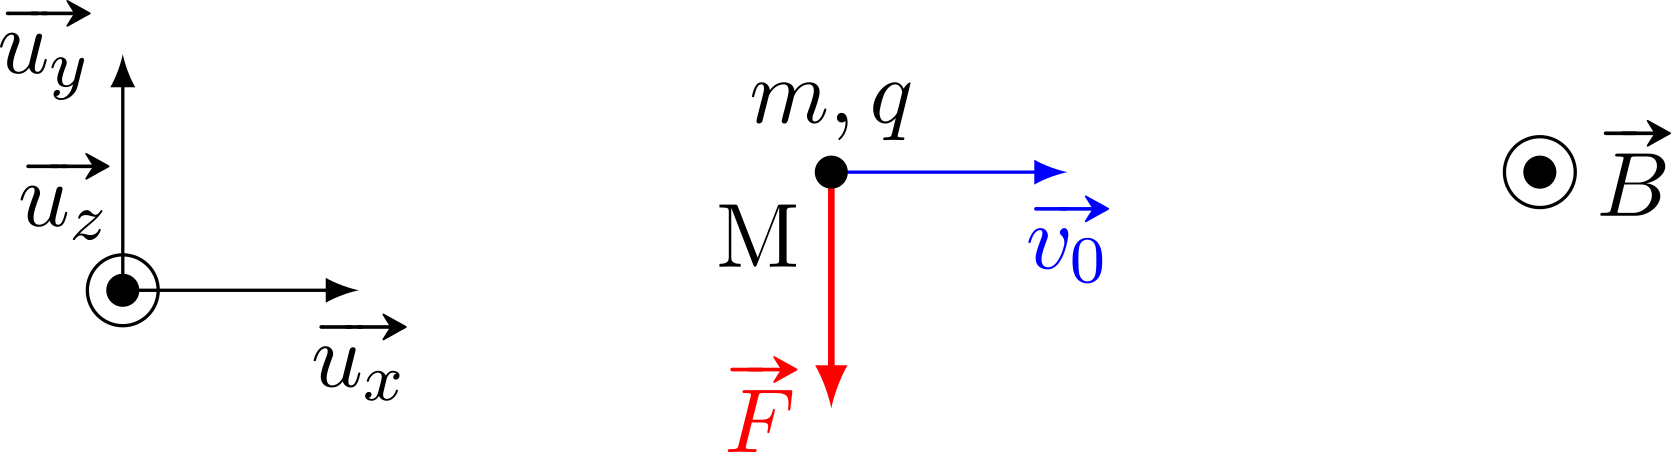
\includegraphics[scale=1, draft=true]{chp_B-base}
		}{
			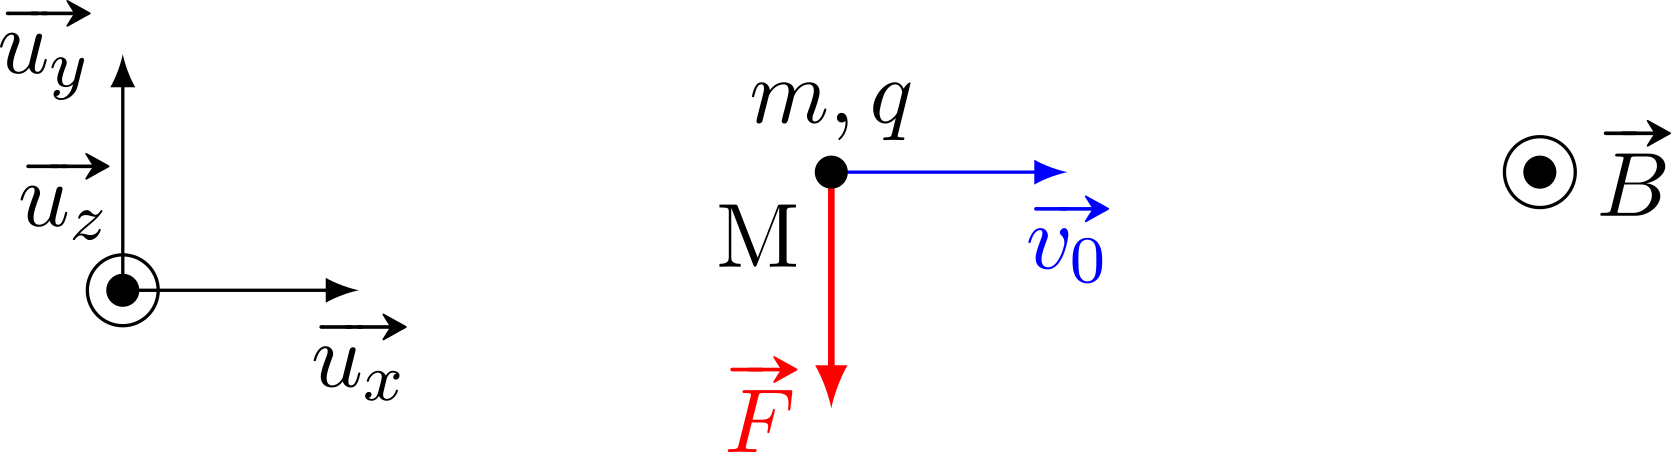
\includegraphics[scale=1]{chp_B-base}
		}
		\psw{
			\[
				\begin{array}{ll}
					\textbf{Poids}            & \text{négligeable \textbf{devant }}\Ff \\
					\textbf{Force magnétique} & \Ff = q\vf\wedge\Bf =
					\mqty(q\xp                                                         \\q\yp\\q\zp)\wedge\mqty(0\\0\\B)\\
					\Lra                      & \Ff = q\yp B\ux -q\xp B\uy
				\end{array}
			\]
			\begin{gather*}
				m\af = \Ff \Lra
				\left\{
				\begin{aligned}
					m\xpp & = q\yp(t)B  \\
					m\ypp & = -q\xp(t)B \\
					m\zpp & = 0
				\end{aligned}
				\right.
				\Lra
				\left\{
				\begin{aligned}
					\xpp(t) & = \frac{qB}{m}\yp(t)  \\
					\ypp(t) & = -\frac{qB}{m}\xp(t) \\
					\zpp(t) & = 0
				\end{aligned}
				\right.
				\Ra
				\left\{
				\begin{aligned}
					\xp(t) & = \frac{qB}{m}y(t) + v_0 \\
					\yp(t) & = -\frac{qB}{m}x(t) + 0
					\zp(t) & = 0
				\end{aligned}
				\right.
			\end{gather*}
		}
		\tcblower
		\begin{gather*}
			\beforetext{Or, par TPC}
			\Ec_c = \cte \Lra v_x(t)^2 + v_y(t)^2 = \cte = v_0{}^2
			\\\Ra
			\left(\frac{qB}{m}y(t) + v_0\right)^2 + \left(-\frac{qB}{m}x(t)\right)^2 =
			v_0{}^2
		\end{gather*}
	\end{isd}


	\ifstudent{
		\begin{tikzpicture}[remember picture, overlay]
			\node[anchor=north west, align=left]
			at ([shift={(1.4cm,0)}]current page.north west)
			{\\[5pt]\Large\bfseries Nom~:\\[10pt]\Large\bfseries Prénom~:};
			\node[anchor=north east, align=right]
			at ([shift={(-1.5cm,-17pt)}]current page.north east)
			{\Large\bfseries Note~:\hspace{1cm}/20};
		\end{tikzpicture}
	}
\end{enumerate}
\end{document}
